\Chapter{A direkt és az inverz feladat megoldási módszerei}
\label{ch:concept}

A dolgozat témájának megértéséhez érdemes betekintést nyerni a kiinduló, direkt problémába is, vagyis az objektumfelismerés témakörébe. Mivel ennek az irodalma is igen szerteágazó és igazán változatos irányokban történnek a kutatások, így csupán egy rövid áttekintő betekintést kíván nyújtani a dolgozat erre vonatkozó alfejezete.

Az inverz problémakörbe való betekintés az aktuális eredmények ismertetésével történik, amely segítséget nyújthat az inverz probléma kutatási irányainak megértésében is. A dolgozat során kialakított saját megoldásom architekturális vázlata is bemutatásra kerül a fejezetben, amelyet az irodalomkutatás során szerzett tapasztalataim által alakítottam ki, így az aktuális eredmények ismeretében remélhetőleg könnyebben átláthatóak lesznek a kutatási folyamataim az Olvasó számára.

Ezen fejezetben kerül ismertetésre továbbá a megvalósításhoz használt fejlesztői eszközök és a gépi tanulásra épülő modellek tanításának módjai is.

\Section{Az objektumfelismerés}

Az objektumfelismerés célja a számítógépes látás esetében az, hogy egy gépi tanulásos modell egy vizsgált képen meghatározza az azon található objektumokat. Egyszerűbb esetben osztályozási feladatról beszélhetünk, amely során a bemeneti képeket egy-egy címkével látja el a modell. Kimeneteként rendszerint az osztályokhoz tartozó valószínűségi értékeket kaphatjuk meg. Amennyiben a képen található objektum környezetéről feltételezzük, hogy nem hordoz számunka lényeges információkat, úgy a címkék használata elegendő lehet bizonyos feladatoknál. Viszont előfordulhat olyan alkalmazási környezet is, amikor a bemeneti képeken nem csupán egyetlen objektum található, és minden fellelhető objektumhoz szeretnénk címkét rendelni. Ilyen esetekben a felismert objektumokat különféle annotációkkal láthatja el a modell. Legtöbbször a megtalált objektumok pozícióiról is adhat kimenetet, az azonosított elemeket befoglaló dobozokkal  (\ref{fig:yolo}. ábra) \cite{redmon2016you}, vagy pixel-szinten is jelölheti a modell. Az utóbbi esetben szemantikus szegmentációról beszélhetünk \cite{long2015fully}.

\begin{figure}[h]
	\centering
	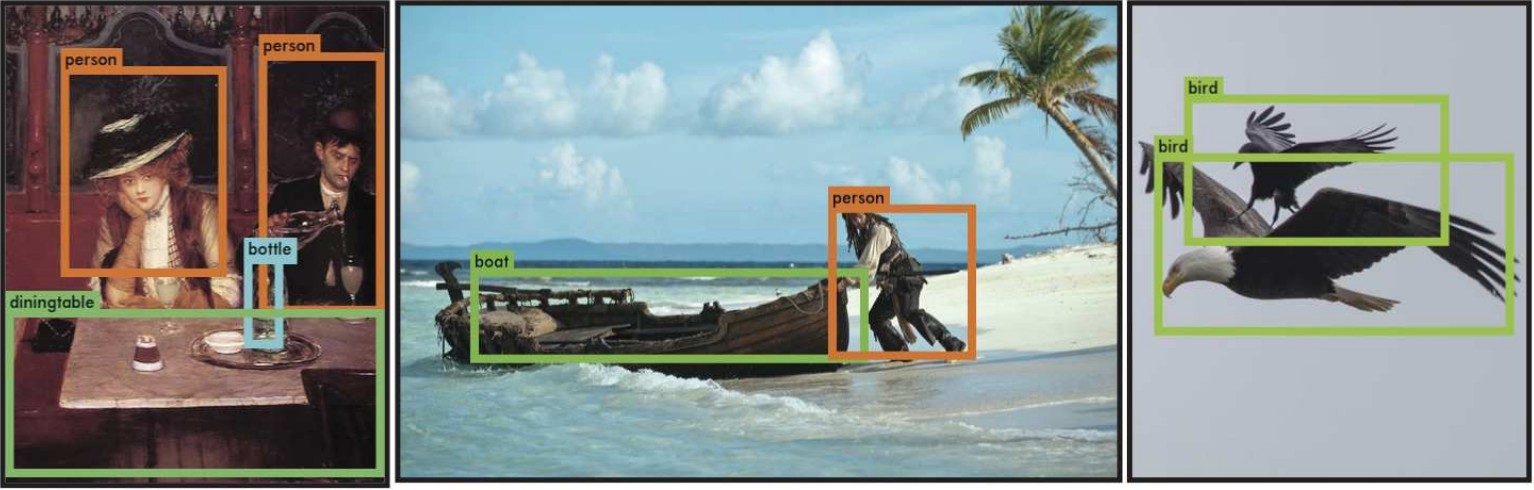
\includegraphics[width=15cm]{images/yolo.png}
	\caption{A YOLO osztályozó által megtalált befoglaló dobozok. \textit{Forrás:} \cite{redmon2016you}}
	\label{fig:yolo}
\end{figure}

A képek osztályozásához többségében \textit{konvolúciós} hálózatot szokás alkalmazni. A konvolúciós rétegeket tartalmazó modell ezen rétegek segítségével nyeri ki az osztályozási művelet elvégzéséhez szükséges képi-jellegzetességeket. A digitális képek $n \times m$-es mátrixokként vannak reprezentálva, a mátrix egyes pontjai pedig szürkeárnyalatos képek esetében a pixel intenzitásának értékei, színes képek esetén pedig az adott színkeverés alapján a színcsatornák értékei. A konvolúciós rétegek a kernelek és a filterek segítségével oly módon nyerik ki a bemeneti képek jellegzetességeit, hogy figyelembe veszik a pixelek környezetét és a céljuk az, hogy a képeken található információt egy kisebb dimenziószámú reprezentációba transzformálják. A kisebb dimenzióban reprezentált adatokon az osztályozási feladat egyúttal könnyebben elvégezhető, másfelől a megfelelően összeállított jellegvektorok segítségével a képen található információ általánosabb formáját kapja meg az osztályozó, csökkentve annak a veszélyét, hogy a modell jellegtelen pixelekre tanulja be az egyes osztályokat.

Kiemelném az \textit{Inception modell}-t \cite{szegedy2015going}, amely a Google kutatói által kifejlesztett mély konvolúciós hálózat. Fő céljuk egy olyan modell megalkotása volt, amely az \textit{ImageNet} adathalmaz \cite{deng2009imagenet} 1000 darab osztályára megoldja az osztályozási feladatot. Az eredeti modell 2014-es megjelenése óta három további verziót is megélt (v2/v3 \cite{szegedy2016rethinking}, v4 \cite{szegedy2017inception}). A modell az inverz probléma egyes megoldásai során is szerepet kap, így a dolgozatban a későbbiekben is említésre kerül.

Az irodalomkutatás során fellelt eredmények közül a legfigyelemreméltóbb eredmény a CLIP \textit{zero-shot} osztályozó \cite{radford2021learning}, amelyet az internetről összegyűjtött képeken és a hozzájuk tartozó szöveges leírásokon tanítottak be. A CLIP modell képes rövid leírásokat adni a kép tartalmáról és az egyes mondatokat valószínűségi értékekkel látja el. Vagyis, a különféle annotációk helyett természetes-nyelvi leírásokat ad kimenetként egy-egy képhez. A modell az inverz problémakör egyes megvalósításában is feltűnik majd, amelyeket a következő alfejezetben ismertetek.


\Section{Az objektumfelismerés inverz problémája}

Az objektumfelismerés inverz problémája alatt azt a feladatot értjük, amely során csupán a képekre vonatkozó információk állnak rendelkezésünkre, és ezen adatok alapján a gépi tanulásos modellnek a lehető legjobban kell reprezentációt találnia egy-egy kimeneti kép formájában.
Ehhez nem csupán a bemeneti, általában természetes nyelvi szöveget kell értelmeznie a modellnek, hanem a kimeneti képek előállításának módja is megoldandó feladat.
A jelenlegi eredmények alapján különféle megközelítéseket láthatunk a problémára, viszont ha csak az eredmények rendezetlen halmazára tekintünk, akkor az aktuális kutatási irányokat nehéz észrevenni. Az eredményeket többféle szempont szerint is csoportosíthatjuk az átláthatóság megkönnyítése érdekében. Mivel a megoldandó probléma alapvetően két részre osztható (a bemeneti adatok feldolgozása és a kimeneti kép előállítása), így első körben a csoportosítást ezen két tengely mentén külön-külön is elvégezhetjük.

\SubSection{Irodalom csoportosítása a kimenet alapján}
Ha a kimeneti képek alapján szeretnénk csoportosítani a jelenlegi eredményeket, akkor megállapíthatjuk, hogy a legtöbb szerző fotorealisztikus megjelenítésre törekedett. A képek előállítására általában \textit{generatív} modellt alkalmaztak, amely a gépi tanulásos megoldások azon halmaza, melynek feladata, hogy új adatokat állítsanak elő. Két generatív modell alkalmazása figyelhető meg a jelenlegi kutatási irányokban.
A képek kigenerálásához vagy \textit{Variational Autoencoder} (VAE) architektúrán alapuló modellt alkottak meg \cite{ramesh2021zero}, vagy \textit{Generative Adverserial Network} (GAN) alapú megoldásokat \cite{dong2021unsupervised, reed2016learning, xu2018attngan, zhang2017stackgan} alkalmaztak.

\begin{figure}[h]
	\centering
	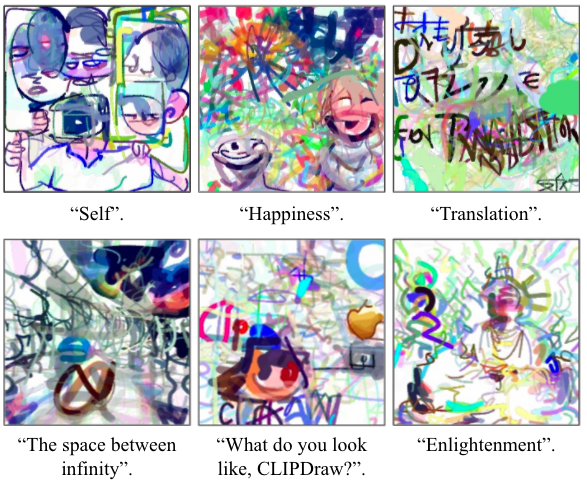
\includegraphics[width=8cm]{images/clipdraw.png}
	\caption{Példák a ClipDraw kimeneteire. \textit{Forrás:} \cite{frans2021clipdraw}}
	\label{fig:clipdraw}
\end{figure}

Egy olyan publikációt is találtam, amely figyelemreméltó módon nem generatív modellt alkalmazott a képek szintetizálására, hanem teljesen egyedi megközelítést, amelyben csupán Bézier-görbék halmazán végezték el az optimalizálást, és eredményül rajzokhoz hasonló képeket kaptak. A módszert \textit{CLIPDraw}-nak nevezték el \cite{frans2021clipdraw}, amelynek a nevében megtalálható, a már korábban említett CLIP osztályozó is. A módszer által előállított kimenetekre \aref{fig:clipdraw}. ábrán találhatók példák.

A GAN és VAE részletesebb összehasonlítására egy későbbi fejezetben kerül sor. A saját módszeremhez szükséges képek előállítására szolgáló komponens alapjául, a különféle eredmények és a két módszer előnyeinek és hátrányainak figyelembe vételével úgy döntöttem, hogy a GAN modellt választom.
A GAN-hoz is igen szerteágazó kutatási irányok alakultak ki az évek során, amelyekben a közös cél természetesen az eredeti GAN kiegészítése oly módon, hogy a betanított modell a lehető legjobb eredményeket nyújtsa. A tanítás stabilabbá tételére vonatkozó kutatások valójában a generált képek fotórealisztikusabbá tételével együtt fejlődtek.

\begin{figure}[h]
	\centering
	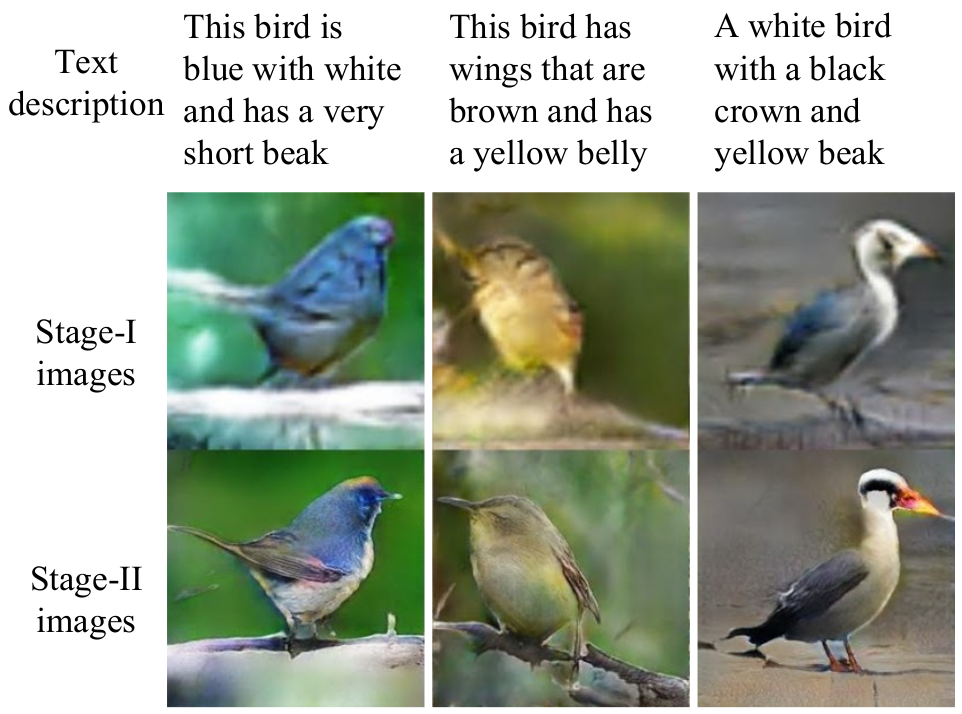
\includegraphics[width=8cm]{images/stackGAN.png}
	\caption{Példák a StackGAN kimeneteire. \textit{Forrás:} \cite{zhang2017stackgan}}
	\label{fig:stackgan}
\end{figure}

A felbontás növelésére például a \textit{StackGAN} \cite{zhang2017stackgan} kétszintű GAN modellt használ: az első szinten alacsonyabb felbontáson kerül kigenerálásra egy kép a bemeneti zajvektorból, majd egy teljesen független GAN hálózat Generátor bemeneteként fog szolgálni az alsó szint generátorának a kimenete, mint zajvektor. Így a második szinten nagyobb felbontásban is ki tud generálódni a megfelelő kép. A StackGAN kimeneteire \aref{fig:stackgan}. ábrán látható példa.
A \textit{ProGAN} \cite{karras2017progressive} architektúra úgy oldotta meg az felbontás növelést és a globális összefüggőség (koherencia) biztosítását, hogy a modellt alacsony felbontáson kezdték tanítani, majd ha betanult az adott felbontásra a modell, új rétegekkel bővítették ki, így növelve a felbontást. Az alacsonyabb felbontáson betanult jellegzetességek a további tanítási fázisokban kiegészítésekre kerültek a magasabb felbontásokon. A ProGAN ihlette a \textit{Multi-Scale Gradient GAN} \cite{karnewar2020msg} architektúrát is, amelynek szintén a felbontásnövelés és a képek részletességének növelése volt a célja. A ProGAN-al ellentétben a Multi-Scale Gradient GAN architektúráját a tanítás során nem szükséges módosítani, ugyanis a Generátor több kimenettel rendelkezik, amelyen ugyanazon generált kép különféle felbontásai találhatóak, míg a Diszkriminátor több bemeneten várja a képeket, különböző felbontások mellett. Az architektúra némileg hasonlít az \textit{U-net}-hez \cite{ronneberger2015u}. A technika nem csupán részletes képeket ígér, de mindemellett a tanítást is stabilabbá teszi.

\SubSection{Irodalom csoportosítása a bemenet feldolgozása alapján}

A megjelenítésen túl a szöveg feldolgozásában is tehetünk különbségeket. Az irodalomkutatás során talált munkákban a bemenet természetes nyelvű szövegként kerül megadásra. Az elsődleges szempont jelen esetben az, hogy a bemeneti szöveg tartalmát minél jobban visszaadja a kép vizuálisan is, így olyan megoldásokra van szükség, amellyel ezt biztosítani lehet. A bemeneti szöveg általában csupán egyetlen leíró mondat, amely a képre vonatkozó információkat magában foglalja, és ami alapján a megjelenítendő képet el kell készíteni.

Egyik megoldásként a \textit{label-conditioning} \cite{mirza2014conditional} technika kerül alkalmazásra a bemenet \textit{embedding} technikával transzformált változatával. Az embedding elkészítése során szempont lehet az is, hogy a hasonló jelentésű szavak közel kerüljenek az embedding terében. Ennek hatására a hasonló embedding vektorral rendelkező mondatokra hasonló képek kerülnek kigenerálásra. A technikát \textit{Conditioning Augmentation}-nak is nevezik \cite{reed2016learning, zhang2017stackgan}.

Mivel a téma a \textit{Natural Language Processing} (NLP) témakörével is összefügghet a bemenet irányából, így az onnan ismert technikák is alkalmazásra kerülhetnek.
Az \textit{Attngan} \cite{xu2018attngan} szövegkódolója például egy \textit{bi-directional Long Short-Term Memory} (LSTM), amely a bemeneti szöveget komponensei szerint vizsgálja. A hivatkozott cikkben fontosnak találták a szerzők, hogy a modell a mondat lényegi részeit a lehető legpontosabban jelenítse meg. Vagyis, a generálás ebben az esetben egy többlépcsős folyamat, amely során a fontosabb szavak által hordozott jelentés kigenerálódik a képen a megfelelő pozíciókra, ezzel is növelve a kép pontosságát. Az attention mechanizmusra még abban az évben érkezett egy igen nagy jelentőségű megoldás, amelyet \textit{transformer} architektúrának \cite{vaswani2017attention} neveztek el, amely egy új irányt jelölt ki az NLP nyelvi modellek világában. A DALLE \cite{ramesh2021zero} nyelvi modelljének alapját is a transzformer architektúra adja. \Aref{fig:dalle}. ábrán figyelhejük meg a DALLE modell kimeneteit.

\begin{figure}[h]
	\centering
	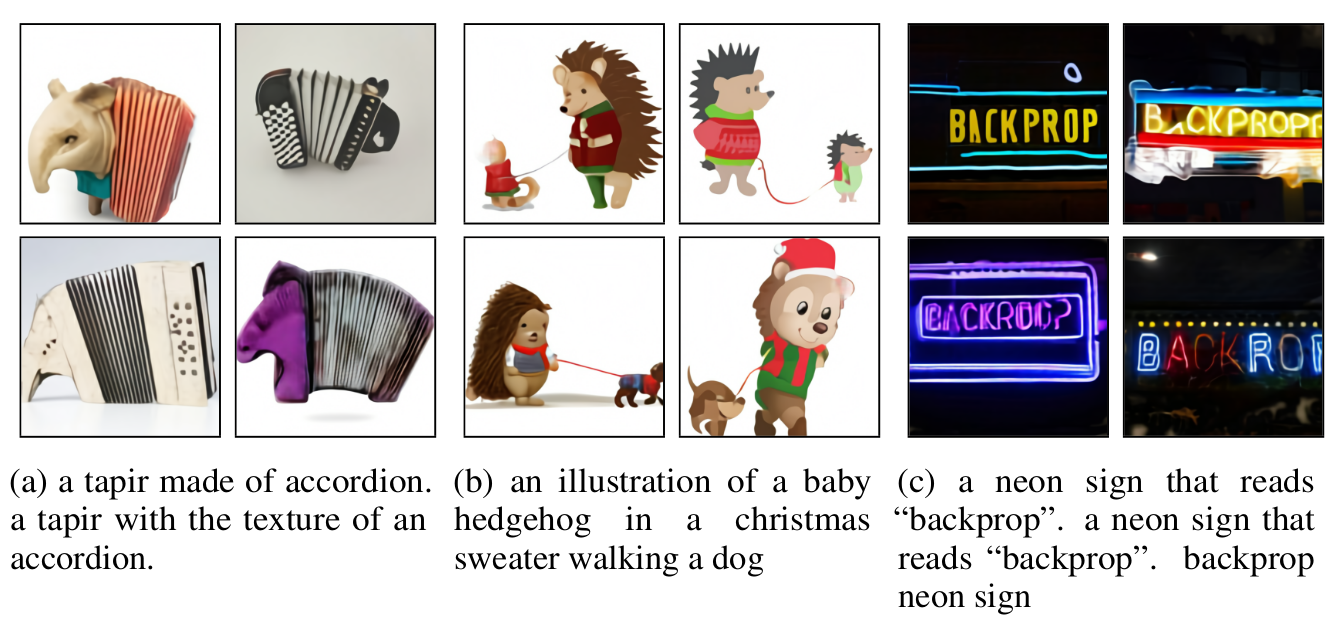
\includegraphics[width=13cm]{images/dalle.png}
	\caption{Példák a DALLE kimeneteire. \textit{Forrás:} \cite{ramesh2021zero}}
	\label{fig:dalle}
\end{figure}

Egy külön csoportként kezelhetjük azokat a megoldásokat is, amikor nem a generáló modellben van beépítve a szövegfeldolgozás, hanem a szöveg és a gép együttesen van felhasználva egy olyan optimalizáláshoz, amelyet egy külső osztályozó segítségével hajtanak végre. Az ilyen módszereket \textit{synthesis-through-optimization} módszereknek \cite{frans2021clipdraw} is nevezhetjük. A ClipDraw cikk a betanított CLIP zero-shot osztályozót használja fel az optimalizáláshoz. A bemeneti szöveget dekódolják és egy véletlenszerűen generált görbehalmazzal indul az algoritmus. A cél az, hogy a gradiens módszer alkalmazása során minimalizálja a bemeneti szöveg kódja- és a CLIP osztályozó által kiadott eredmény közötti koszinuszi távolságot.

\Section{A saját architektúra áttekintése}

A kutatásom során szerzett ismeretek alapján \aref{fig:architecture}. ábrán szemléltetett architektúrát alkottam meg.

\begin{figure}[h]
\centering
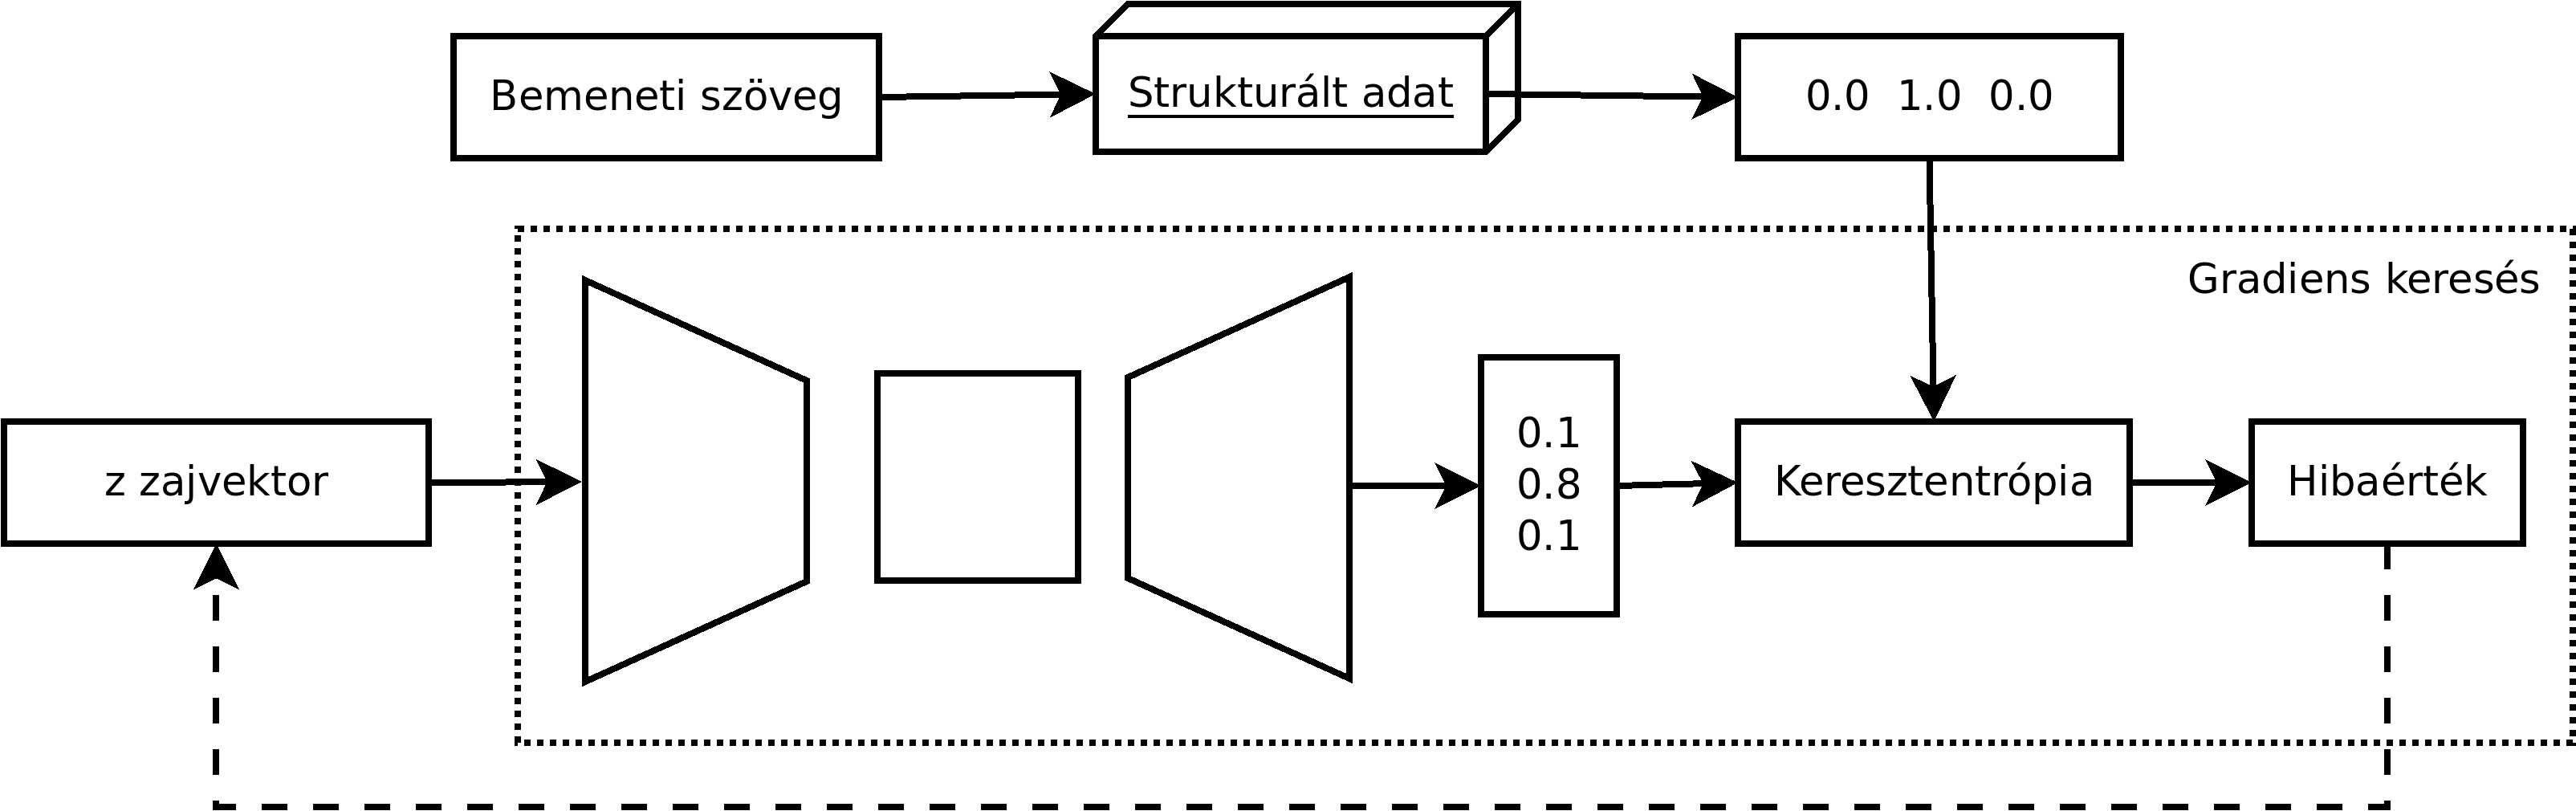
\includegraphics[width=15cm]{images/architecture.png}
\caption{A probléma megoldásához összeállított architektúra}
\label{fig:architecture}
\end{figure}

Az architektúra részei az alábbiak:

\begin{itemize}
	\item Bemeneti szöveg feldolgozó,
	\item Strukturált adat enkódoló,
	\item Optimalizáló modul:
		\begin{itemize}
			\item Optimalizálandó zajvektor,
			\item Képeket előállító háló (G),
			\item Osztályozó (D),
			\item Hibafüggvény számoló.
		\end{itemize}
\end{itemize}

Az architektúra működése az említett \textit{synthesis-through-optimization} módszeren alapszik. Az optimalizálás célja egy olyan zajvektor keresése, amely a képeket kigeneráló háló bemeneteként a megfelelő képet előállítja.
A megoldásom egyes részei különféle megközelítési módszereken keresztül kerülnek ismertetésre a dolgozat további fejezeteiben.

%TODO: Részletezés kicsit?

\Section{A Tensorflow és Keras függvénykönyvtárak}

A dolgozat programjának megvalósításához a TensorFlow függvénykönyvtárat választottam ki. A TensorFlow egy ingyenes, nyílt forráskódú gépi tanulásra használatos függvénykönyvtár, amely elsősorban mély- és gépi-tanulásos alkalmazások implementálására használatos. Számos programozási nyelvhez érhető el az API-ja, beleértve a Python, Java, C++ és JavaScript nyelveket. Az API fő fejlesztési iránya a Python nyelvre összpontosul. A könyvtár a Google Brain fejlesztésében született meg 2015-ben, majd 2019-ben megjelent a 2.0-ás API verzió is, amely az API váltásból adódóan visszafelé nem teljesen kompatibilis az elsővel. Jelenleg a 2.8-as számozású stabil kiadással rendelkezik, melynek dokumentációja a \cite{tensorflow} forrás alatt érhető el. Az API lehetőséget ad az elosztott tanításra is. A betanított modellek széles körben alkalmazhatóak, akár web- vagy mobilalkalmazásokba is integrálhatóak. 

A Keras függvénykönyvtár egy interfészt biztosít a TensorFlow-hoz. Segítségével igazán egyszerűen, modulárisan és átláthatóan állíthatunk össze neurális hálózatokat. Az általa biztosított eszközkészlet igazán változatos és kifejező. A modellek összeállítására is többféle lehetőségünk van, például a \textit{Sequential API} használatával pipeline szerű modelleket építhetünk a különféle rétegek egymás után illesztésével. A \textit{Functional API} segítségével pedig komplex kapcsolatokkal rendelkező architektúrák is megvalósíthatóak, a kódbonyolultság növekedése nélkül. A Keras korábban több backend-et is támogatott, viszont a legfrissebb verzióiban csak a TensorFlow-hoz alkalmazható. Látható, hogy a két könyvtár mennyire összefonódott. A dokumentációja a \cite{keras} forrás alatt érhető el.

Python-ban a \texttt{tensorflow} csomag az alábbi kódrészlettel importálható. A TensorFlow tartalmazza a Keras-t is modul formájában. Amennyiben nem importáljuk be külön a modult, úgy a \texttt{tf.keras}-al is elérhetjük, viszont az alábbi kódrészletben a Keras is importálásra kerül. A dolgozatban található kódrészleteknél az alábbi két sort nem tüntetem fel a továbbiakban, egységesen minden kódrészlethez az alábbiak szükségesek. (A kivételt képző eseteknél, ahol szükséges lehet további csomagok importálása is. Ezeket külön ki fogom emelni.)
\begin{python}
import tensorflow as tf
from tensorflow import keras
\end{python}

A dolgozathoz elkészült programok \textit{IPython Jupyter notebook}-ok \cite{jupyter} formájában kerültek megvalósításra.

\Section{A tanításhoz használt adathalmazok}

A tanításhoz szükségünk van egy megfelelő adathalmazra. Képek generálásához legegyszerűbb esetben elegendő lehet képek rendezetlen halmaza is, és a modellre bízhatjuk, hogy ismerje fel az egyes osztályok jellegzetességeit. Megfelelő regularizációs technikákkal igazán változatos képek generálására lesz képes a betanított modell a megfelelő adathalmazon.

Ha az adathalmaz rendelkezik osztályokkal is, úgy az osztály-címkéket is felhasználhatjuk a GAN hálózatunk tanításához. Így egy plusz bemenet segítségével könnyebben tudunk majd megfelelő képeket előállítani. Ezt a technikát \textit{class-conditioning}-nak nevezik.

Egyes adathalmazokhoz igen részletes annotációkat is mellékelnek. A képeken megfigyelhető objektumokat határoló dobozokkal, vagy pixel szinten is jelölik. Így igen részletes információkat kínálnak a kép tartalmáról. Hasznos annotációk lehetnek a természetes nyelvű leíró mondatok is, amelyekből általában többet is mellékelnek egy-egy képhez.

Egyes eredményeknél megfigyelhető, hogy a tanítás során az adathalmaz tisztítására is nagy gondot fordítottak. Például az olyan GAN modelleknél, amelyeknél a felbontás növelését tűzték ki megoldandó problémaként. Az ilyen modelleknél egy széles körben alkalmazott adathalmaz a CELEB FACES, amely hollywoodi hírességek portréit tartalmazza. Az adathalmaz elemeit erősen módosították a szerzők, például a szemeket és az egyéb arci jellegzetességeket pozicionálták minden egyes elemnél.
Ha a modellt olyan adathalmazra tanítjuk, amelyben hasonló objektumok találhatóak, akkor az így betanított GAN-okat témakör specifikusnak (\textit{domain specific}) is nevezhetjük, hiszen a tudása csupán egy-egy osztály objektumaira korlátozódik. Egy-egy valós objektumot többféleképpen is le tudunk fényképezni és ezáltal leképezni egy két dimenziós térre, így a GAN modellnek az is segítség lehet, ha csak olyan képeket mutatunk neki a tanítás során, amelyeket fix pozíciókból fényképeztünk. Az általánosítás szempontjából ez egy nagy könnyítés lehet a modellnek.
Tehát a fotórealisztikus eredményeket elérő modellek esetén kijelenthetjük, hogy nagy szerepe van a megfelelő adathalmaznak is.

Példaként tekintsük az alábbi két adathalmazt.
\begin{itemize}
	\item Animal Faces-HQ (AFHQ) \cite{choi2020stargan} adathalmaz állatokról készített portrékat tartalmaz igen jó minőségben. A színes fényképek felbontása $ 512 \times 512 $, az állatok fotói pedig pozicionálva vannak a szemük szerint. Tehát igen tisztának lehet nevezni az adathalmazt. A dataset-et bevezető publikációban azt is megemlítik, hogy kézi szelektálást is végeztek, hogy a lehető legjobb minőségűek legyenek a minták. A mintákat 3 osztályban adták meg, úgy mint: kutya, macska és vadállat. Az osztályokban egyenként 5000 tanítóminta található, így összesen 15 ezer képből áll az adathalmaz. A kevés osztály ellenére az osztályokon belül igen változatos képek figyelhetők meg, a fajok különböző alfajaira. Néhány példát láthatunk \aref{fig:afhq_dataset_samples}. ábrán.
	
	\begin{figure}[h]
		\centering
		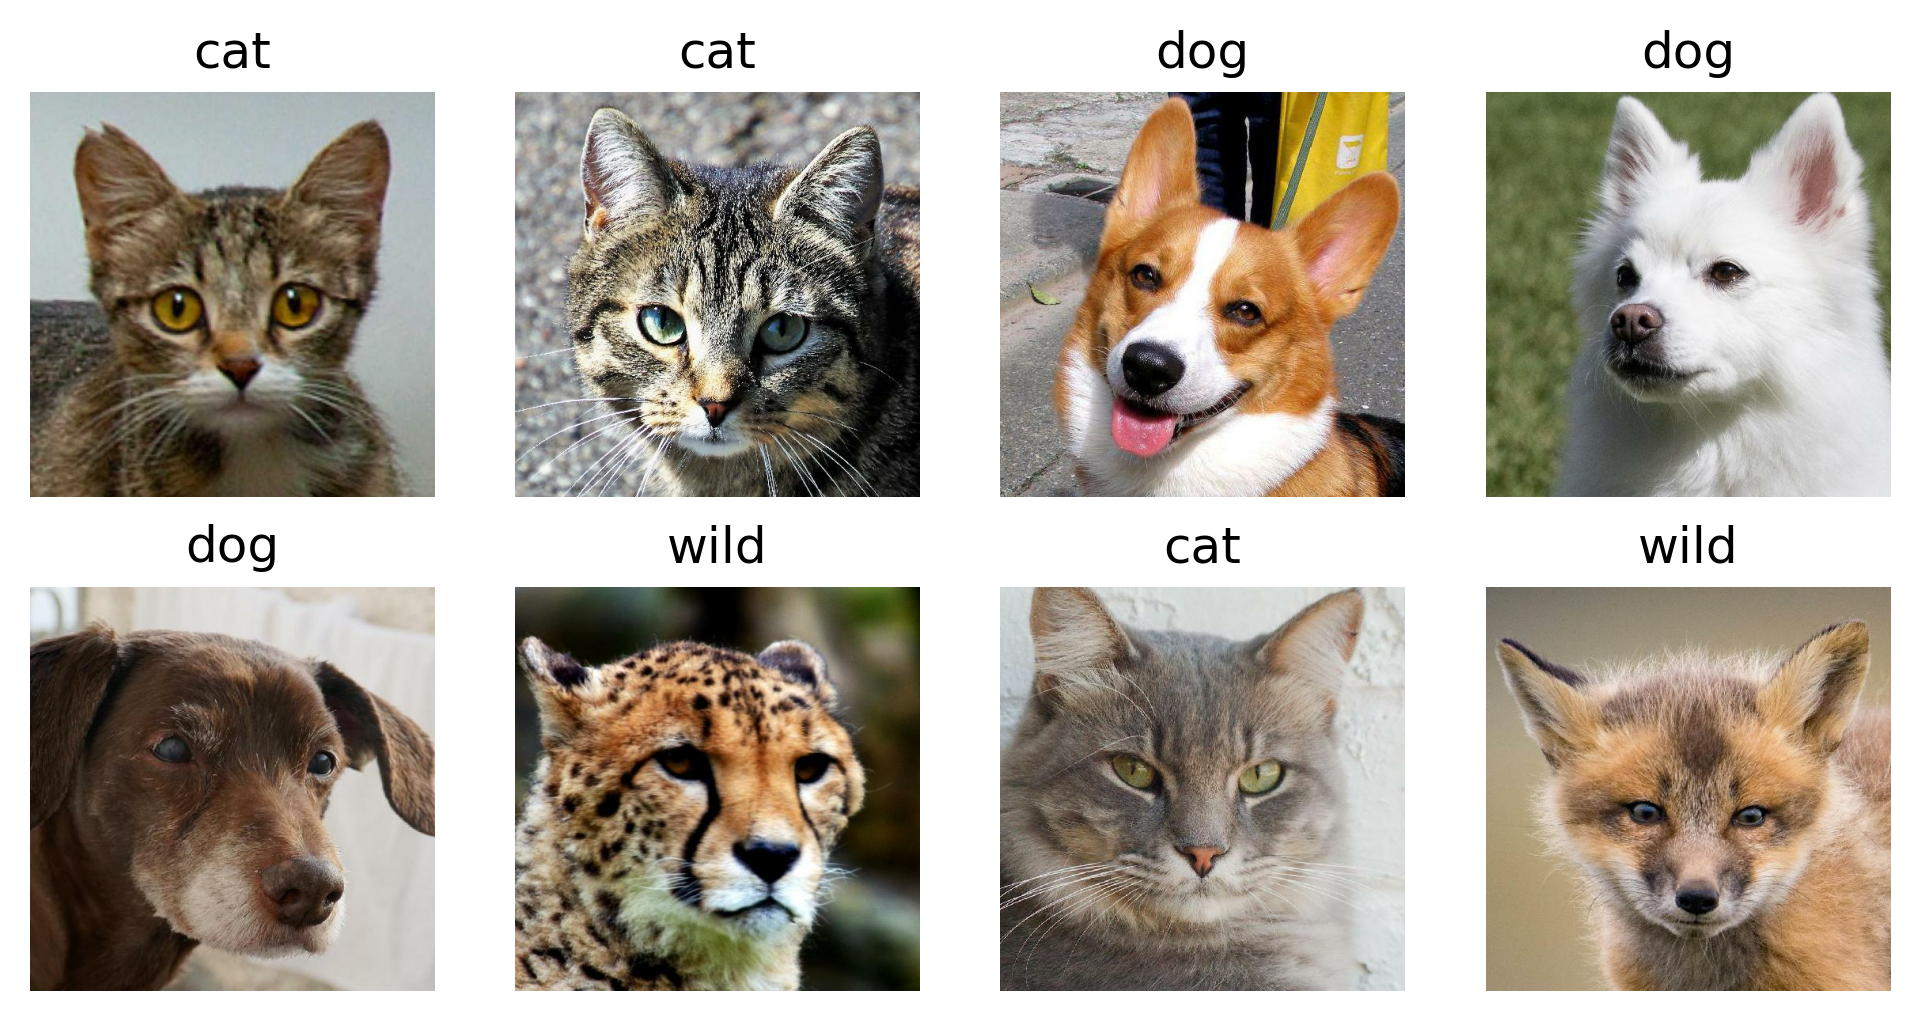
\includegraphics[width=10cm]{images/afhq_dataset_samples.png}
		\caption{Minták az AFHQ adathalmazból. \textit{Forrás:} \cite{choi2020stargan}}
		\label{fig:afhq_dataset_samples}
	\end{figure}
	
	\item A Cifar-10 \cite{krizhevsky2009learning} adathalmaz valójában a Cifar-100 adathalmaznak egy leszűkített változata. Az utóbbi 100 osztályt magába foglaló adathalmaz, míg a Cifar-10 csupán 10 osztállyal rendelkezik. A tanítóhalmaza 50000 képet tartalmaz.
	Az adathalmaz képei ($32 \times 32$) felbontásúak és 3 színcsatornával rendelkeznek (RGB). Néhány példa látható \aref{fig:cifar10_dataset_samples}. ábrán.
	
	\begin{figure}[h]
		\centering
		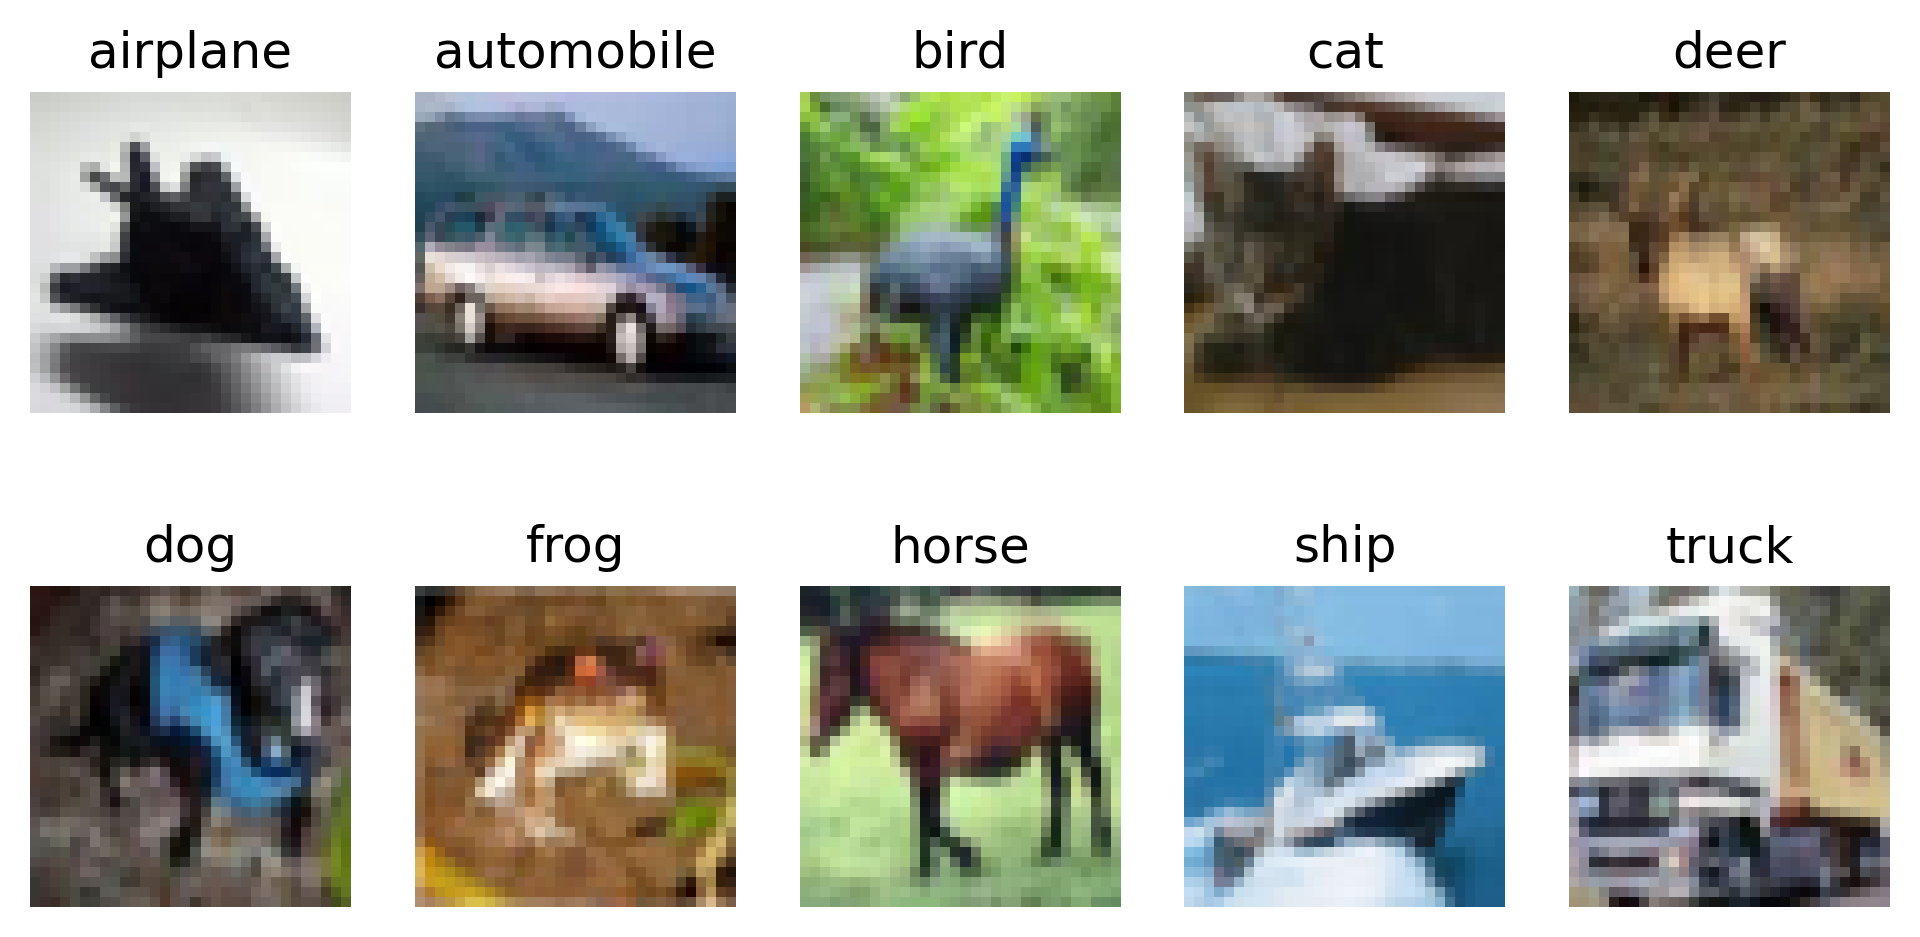
\includegraphics[width=10cm]{images/cifar10_dataset_samples.png}
		\caption{Minták a Cifar10 adathalmazból. \textit{Forrás:} \cite{krizhevsky2009learning}}
		\label{fig:cifar10_dataset_samples}
	\end{figure}
\end{itemize}

\Section{Modellek tanítása}

A mély neurális hálózatok tanítása igazán erőforrás-igényes feladat. A tanítható hiperparaméterek nem ritkán milliós nagyságrendűek, a dataset-eknek pedig kellően nagynak kell lenniük, a feldolgozandó adatoknak pedig memóriába is bele kell férnie. Egy-egy iteráció igen sok időbe telhet egy gyengébb hardveren.

A kezdeti demóprogramok futtatása során szembesültem az első technikai nehézséggel. A laptopom nem volt a legalkalmasabb nagyobb gépi-tanulásos modellek tanítására, hiszen igen sok időt vett igénybe a legkisebb példák futtatása is. Megoldásként egy olyan szolgáltatást kerestem az interneten, amellyel a dolgozatom programjához történő modelleket kényelmesen be tudtam tanítani.

A TensorFlow honlapján felleltem a Google Colab \cite{colab} felületet, amely ingyenes virtuális környezetet biztosít az IPython munkafüzetek szerkesztéséhez és futtatásához. A felület egy előre meghatározatlan ideig GPU-t (Tesla K80) és TPU-t is biztosít kipróbálás jelleggel. Az ingyenes verzióban a napi GPU használatának limitje nincsen meghatározva, így egy idő után lekapcsolhatják és GPU nélkül megnövekszik a tanítás hossza. Továbbá a környezetet 12 óránként újraindítják, így minden adat elveszhet és csak akkor futhat a szkript, ha meg van nyitva a böngészőablak. Így az ingyenes verzió csupán kisebb példák futtatására elegendő. Természetesen a Tensorflow és a Keras ajánl lehetőségeket a modellek mentésére vagy a tanítás közbeni checkpoint-ok készítésére.

Például az alábbi kódrészlet futtatásával tetszőleges attribútumokkal létrehozhatunk egy \texttt{Checkpoint} típusú objektumot, amely segítségével mentéseket csinálhatunk a checkpoint paramétereiként megadott objektumok állapotairól. Ha esetleg a kimentett állapotokat vissza kívánjuk állítani, úgy a \texttt{checkpoint.restore} függvénnyel, és a megfelelő fájlnév megadásával megtehetjük.
\begin{python}
checkpoint = tf.train.Checkpoint(
    generator_optimizer=generator_optimizer,
    discriminator_optimizer=discriminator_optimizer,
    generator=generator,
    discriminator=discriminator
)
checkpoint.save(file_prefix)
checkpoint.restore(checkpoint_path)
\end{python}

Egy másik lehetőségként lementhetjük a teljes modellt, amelyet később egyszerűen be is tölthetünk.
\begin{python}
model.save("./my_model")
new_model = keras.models.load_model("./my_model")
\end{python}
Ennek a módszernek az előnye, hogy nem szükséges a modellt üresen deklarálni a betöltéshez, viszont a checkpoint-tal ellentétben a verziók nincsenek automatikusan menedzselve és erről nekünk kell gondoskodni. Az ilyen mentést a már betanított modellekhez javasolt megtenni, míg a checkpoint a tanítás során nyújt lehetőséget a biztonsági mentések készítésére. A saját modelleim tanítása során is felléptek olyan állapotok, amikor a modell a tanítás során használhatatlanná vált. Ilyen esetekben a biztonsági mentésekkel igen könnyedén vissza lehetett állítani az utolsó stabil állapotot.

Számomra a Google Colab ingyenes próbaverziója nem volt teljesen megfelelő, a kiszámíthatatlanság miatt. Az előfizetés még csupán néhány kijelölt országban elérető, így Magyarországon jelenleg nem lehet a fizetős szolgáltatásra feliratkozni, így újabb felületet kellett keresnem.
Egy fórumon böngészve találtam rá a Kaggle \cite{kaggle} felületre, amely hasonló környezetet kínál, mint a Colab. A Kaggle által biztosított virtuális környezet hardvere jobbnak bizonyult a Colab-bal szemben. A GPU használat heti szinten kerül meghatározásra órákban, ami csak a használat során számolódik. Továbbá lehetőséget kínál a notebook-ok ütemezett futtatására is, és a Kaggle-ön megtalálható bármelyik dataset-et könnyedén betölthetjük és használhatjuk. Mindezen előnyök miatt a Kaggle-t választottam a modelljeim tanítására.

Az alábbi táblázatban található meg a laptopom és a Kaggle által biztosított környezet specifikációi:
\begin{center}
\begin{tabular}{@{\extracolsep{6pt}} l r r }
	\hline
	  & \multicolumn{1}{c}{\textit{Dell Insprion-5558}} & \multicolumn{1}{c}{\textit{Kaggle környezet}}\\
	\cline{2-2} \cline{3-3}
	\textbf{CPU} & Intel Core i3-5005U CPU 4x 2.00GHz & Intel Xeon CPU 2x 2.00GHz\\
	\textbf{RAM} & 2x 4GB DDR3 1600 MHz & 15GB\\
	\textbf{GPU} & Intel HD Graphics 5500 (VGA) & Nvidia Tesla P100-PCIE-16GB\\
	\textbf{HDD} & 1TB & 73GB\\
	\hline
\end{tabular}
\end{center}
A három környezet (laptop, Colab, Kaggle) teljesítményét egy általam felállított méréssel vizsgáltam.
A \texttt{RuntimeMeasure.ipynb} notebook használatos a mérés elvégzéséhez.
A teljesítménymérés alapja egy olyan GAN hálózat, amelyet meghatározott paraméterekkel hozunk létre.
A tanítás során az alábbi paraméterek változatlanok:
\begin{center}
\begin{tabular}{@{\extracolsep{6pt}} c c c c }
	\hline
	Látens dimenziószám & mini-batch méret & filterek száma & kernelméret\\
	\cline{1-1} \cline{2-2} \cline{3-3} \cline{4-4}
	100 & 32 & 128 & ($3\times 3$)\\
	\hline
\end{tabular}
\end{center}
A felbontásnövelő rétegek száma a futó paraméter, amelyet 0-tól 3-ig vizsgálunk.

A hálózat felépítése megegyezik a későbbi fejezetben ismertetett architektúrával, egy minimális eltéréssel, ami csupán a $4 \times 4$-es felbontású képek előállításának segítésére vonatkozik. A kiegészítés csupán annyi, hogy \textit{toRGB} és \textit{fromRGB} rétegek kerülnek alkalmazásra. (Ezen rétegek is a későbbi fejezetekben kerülnek ismertetésre.)

A hálózatot 5 epoch-ig tanítjuk az adott felbontásnövelő rétegek mellett, majd az átlagos futásidő kerül lejegyzésre.
A mérés során a hálózatot a Cifar10 \cite{krizhevsky2009learning} adathalmazon tanítottam, labelek nélkül a train részhalmazán.
A mérés egyes állomásain különféle felbontásokban generálja ki a képeket a modell, így a tanítás előtt a tanítóhalmaz képeit is a megfelelő méretekre skálázzuk.

A modell kimenete a felbontásnövelő rétegek számával változik. Ha nem alkalmazunk ilyen réteget, akkor az ($4 \times 4$) felbontású képeket eredményez, majd rendre 1 réteg esetén ($8 \times 8$), 2 rétegnél ($16 \times 16$) és 3 rétegnél pedig ($32 \times 32$) felbontású képek jelennek meg a kimeneten.

\begin{python}
...
for i in range(upsampling_layers):
    hidden = keras.layers.Conv2DTranspose(
        units_per_layer, kernel_size, 2, 'same'
    )(hidden)
    hidden = keras.layers.BatchNormalization()(hidden)
    hidden = keras.layers.ReLU()(hidden)
...
\end{python}

A modell hálózataiban egy-egy for ciklussal megoldhatjuk az említett rétegek hozzáadását a hálók építésénél. A fenti példa kód szemlélteti a generátorban lévő dekonvolúciós réteg hozzáadását.
A notebook-ot futtatva a különböző környezeteken \aref{fig:runtime}. ábrán látható eredmények jöttek ki.

\begin{figure}[h]
\centering
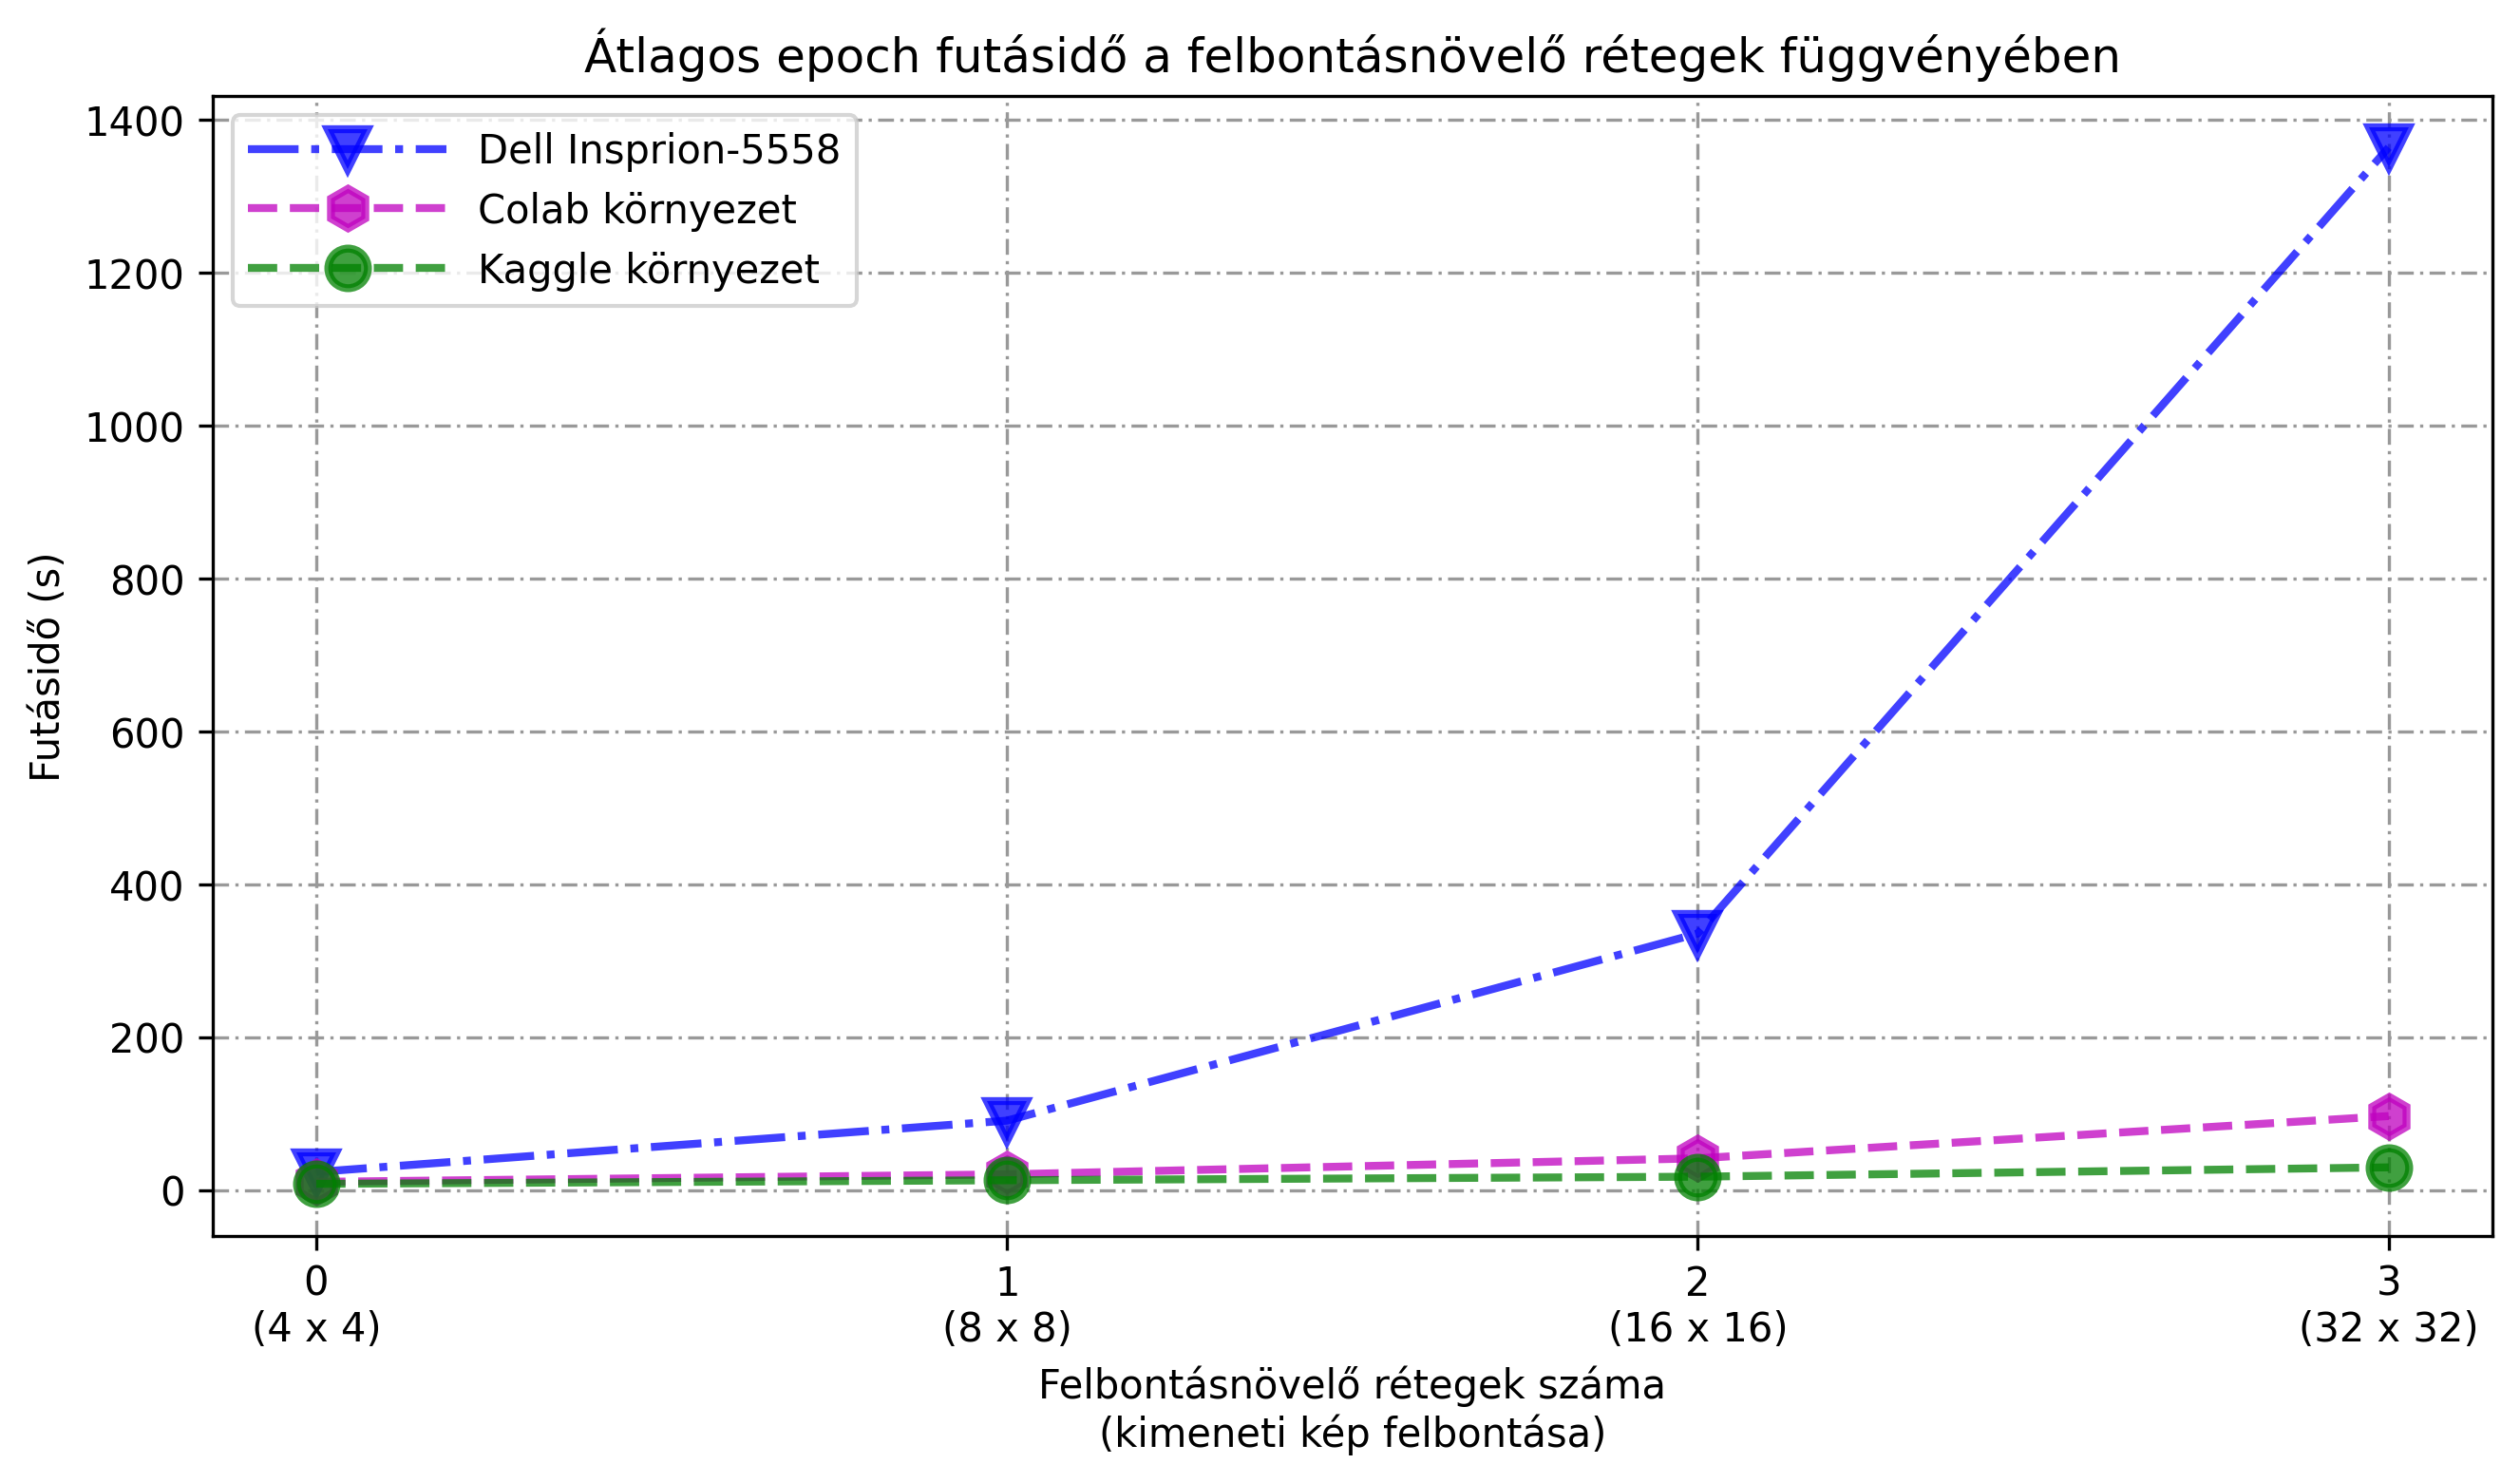
\includegraphics[width=15cm]{images/runtime.png}
\caption{Futási idők a három vizsgált környezetben}
\label{fig:runtime}
\end{figure}

Mint látható, a laptopom igen alulmaradt a két virtuális környezettel szemben, és érzékelteti az ábra, hogy saját munkaálláson mennyire kényelmetlenné válik a tanítás a várakozási idők meghosszabbodásával. A modellek összeállításának kezdeti fázisaiban több prototípus készült el, mire eljutottam a végleges változatig. Az egyes próbálkozások a megfelelő modell kiválasztására a laptopomon nagyon sok időt vett volna el, amely rontotta volna a kutatás hatásfokát is.